\documentclass{standalone}
\usepackage{color}
\usepackage{tikz}
\definecolor{accent}{HTML}{00C853}
\definecolor{gray500}{HTML}{757575}

\usetikzlibrary{arrows}
\tikzstyle{vertice}=[circle, draw=black, fill=gray500, inner sep=1mm]
\begin{document}


\begin{document}
\pagenumbering{roman}\pagestyle{plain}
\pagestyle{fancy}
\lhead{}

\begin{titlepage}
	\begin{minipage}[c]{4em}
		
\includegraphics[width=3em]{res/bk.jpg}
	\end{minipage}
	\begin{minipage}[l]{\textwidth - 4em}
		{\Huge Trường Đại học Bách khoa Hà Nội\par}
		{\large Viện Toán ứng dụng và Tin học}
	\end{minipage}
	\vfill
	\vfill
	\begin{center}
		{\Large Tài liệu toán rời rạc}\par
		{\LARGE Nghiên cứu thực nghiệm về công nghệ mạng}\par
		\vfill
		{\large
			\begin{tabular}{rl}
				{ Giảng viên hướng dẫn}:&TS. Lê Chí Ngọc\\
				{ Sinh viên thực hiện:}& Phùng Anh Hùng\\
				{ Lớp học:} & TN Toán -- tin K62
			\end{tabular}
		}
		\vfill
		{\large Hà Nội, tháng 5 năm 2019}
	\end{center}
\end{titlepage}
\tableofcontents

\chapter{Hệ thống mạng Internet}
\pagenumbering{arabic}
\section{Định nghĩa}
Internet là một mạng lưới phủ trên toàn thế giới, kết nối dữ liệu giữa các máy tính và các thiết bị liên quan. Internet là một “Chuyển mạch gói” (Packet Switched ) dữ liệu mạng, nghĩa là tin nhắn được gửi qua nó được chia thành các gói, các khối dữ liệu nhỏ, chúng được gửi qua mạng và ghép lại hoàn chỉnh ở đầu kia. Định dạng của các gói theo một tiêu chuẩn được gọi là Giao thức Internet (Internet Protocol-IP) và bao gồm một địa chỉ IP trong mỗi gói chỉ định đến đích của gói, nhờ đó mà nó có thể định tuyến chính xác vị trí trên mạng.\par
Thay thế cho mạng “Chuyển mạch gói”  là mạng “Chuyển mạch kênh” (Circuit Switched), ví dụ cơ bản là hệ thống điện thoại. Trong mạng chuyển mạch kênh, các mạch kết nối khi cần, chẳng hạn như khi một cuộc gọi được thực hiện, mạng sẽ phân bổ một mạch cho kết nối này, và chỉ dành riêng cho kết nối đến khi cuộc gọi kết thúc. Điều này hoạt động tốt trong hệ thống gọi thoại, với các cuộc gọi có điểm bắt đầu và kết thúc rõ ràng, tuy nhiên lại kém trong mạng dữ liệu, nơi mà việc truyền dữ liệu thường xuyên xảy ra những sự ngắt quãng, gián đoạn đột ngột. Sử dụng mô hình mạng chuyển mạch gói cho phép máy tính truyền và nhận những dữ liệu không liên tục hoặc ở các tốc độ truyền khác nhau mà không làm tăng dung lượng trên mạng. Bằng cách tách các gói nhỏ hợp lý, mạng cho phép một lượng nhất định các trường hợp lỗi. Không có gì lạ khi các gói biến mất trên Internet và không bao giờ đến đích, chỉ đôi khi là do lỗi phần cứng hay phần mềm, nhưng đa phần là do các gói bị xóa có chủ ý nhàm giảm tắc nghẽn trong những phần đang hoạt động bận rộn của mạng. Khi đó những tin nhắn chia thành nhiều gói sẽ bị mất một vài gói, và chỉ cần gửi lại những gói đã mất để hoàn thành tin nhắn thay vì gửi lại toàn bộ tin nhắn. Có một phần mềm được gọi là Transport Control Protocol (TCP) (Giao thức điều khiển và vận chuyển) chạy trên IP, nó tự động thực hiển kiểm tra và truyền nếu xảy ra lỗi mà không cần đến sự can thiệp từ người dùng máy tính hay một phần mềm nào khác.\par
Đại diện cơ bản nhất cho mạng Internet là các đỉnh của mạng đại diện cho các máy tính và thiết bị liên quan, còn các cạnh thì đại diện cho kết nối giữ chúng. Trên thực tế các máy tính thông thường chỉ chiếm các đỉnh bên ngoài mạng, các dữ liệu truyền đến và đi, chúng không đóng vai trò trung gian cho luồng dữ liệu giữa các mạng khác (Các máy tính thường chỉ kết nối duy nhất với mạng nên không nằm trên đường giữa bất kì máy tính nào khác). Các nút bên trong mạng Internet chủ yếu là các bộ đinh tuyến, máy tính chuyên dụng, nằm tại điểm nối giữa các dòng dữ liệu, chuyển tiếp gói dữ liệu theo hướng về đích dự định của chúng.\par

\section{Cấu trúc Internet dưới dạng sơ đồ}
Hình dạng tổng thể của Internet được hiển thị ở dạng sơ đồ trong hình \ref{fig:h21}. Mạng bao gồm ba cấp vòng tròn. Vòng tròn thứ nhất là cốt lõi của mạng, là xương sống (Backbone) của mạng, các đường trục cung cấp đường truyền dữ liệu băng thông đường dài toàn cầu, cùng với những bộ định tuyến hiệu suất cao, chúng được liên kết với nhau bởi trung tâm chuyển mạch. Backbone được vận hành bởi các nhà cung cấp (NBPs) (network backbone providers), chủ yếu là chính phủ các quốc gia và công ty truyền thông. \par
Vòng tròn thứ hai của mô hình Internet bao gồm các nhà cung cấp dịch vụ Internet hoặc ISPs, các công ty thương mại, chính phủ, trường đại học và những người có hợp đồng với NBPs để kết nối với xương sống và sau đó bán lại hoặc cung cấp kết nối đó cho người dùng, người tạo thành vòng tròn thứ ba, các doanh nghiệp, văn phòng chính phủ, học giả, người trong nhà, v.v. Trên thực tế, như hình \ref{fig:h21} cho thấy, các ISPs được chia nhỏ thành các ISPs khu vực và ISPs địa phương hoặc ISPs tiêu dùng, trước đây các tổ chức lớn có nhiều khách hàng là ISPs địa phương, những người lần lượt bán kết nối mạng cho người dùng. Tuy nhiên, sự khác biệt này có phần mờ nhạt, bởi vì các ISPs tiêu dùng lớn, như America Online hoặc British Telecom, thường hoạt động như các ISP khu vực của riêng họ (và một số cũng có thể là nhà cung cấp xương sống).
\begin{figure}[ht]
\centering
	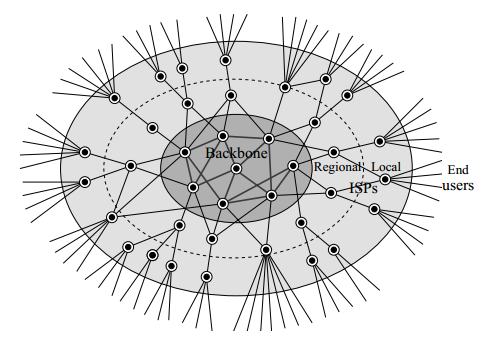
\includegraphics[width=0.5\textwidth]{res/h21.png}
	\caption{sơ đồ cấu trúc Internet: “Backbone”: xương sống của dải băng thông. ISPs: kết nối với “Backbone” và bị chia khoảng bởi Regional (Khu vực lớn) và Local (Địa phương nhỏ). End users: người dùng cá nhân, gia đình, công ty kết nối với ISPs.}
	\label{fig:h21}
\end{figure}

Cấu trúc mạng của Internet không bị quy định bởi bất kỳ cơ quan trung ương nào. Các giao thức và hướng dẫn được phát triển bởi một tổ chức tình nguyện không chính thức có tên là Internet Engineering Task Force, họ không phải nộp đơn cho bất kỳ cơ quan Internet trung ương nào để xin phép xây dựng một mạng mới trên Internet hoặc đưa ra khỏi dịch vụ.\par
Một trong những tính năng đáng chú ý của Internet là sơ đồ được sử dụng để định tuyến các gói từ đích này đến đích khác được đưa ra bằng cách trao đổi tự động giữa các bộ định tuyến Internet bằng cách sử dụng một hệ thống gọi là Giao thức cổng biên (Border Gateway Protocol- BGP). BGP được thiết kế theo cách nếu các đỉnh hoặc cạnh mới được thêm vào mạng, các đỉnh cũ biến mất, các điểm hiện tại bị hỏng vĩnh viễn hoặc tạm thời, các bộ định tuyến sẽ lưu ý và điều chỉnh hệ thống định tuyến của chúng một cách thích hợp. Một số hoạt động cần con người giám sát để đảm bảo sự trơn tru, nhưng không cần có “chính quyền Internet” nào để điều khiển mọi thứ từ trên cao, hệ thống tự tổ chức bằng cách kết hợp hoạt động của hệ thống máy tính địa phương cơ bản tự động.\par
Mặc dù đây là một tính năng tuyệt vời của hệ thống với sự mạnh mẽ và linh hoạt, nhưng nó là một vấn đề đối với những người muốn nghiên cứu cấu trúc của Internet, bởi vì không có đăng ký trung tâm nào mà người ta có thể xác định cấu trúc đó. Không có ai có nhiệm vụ duy trì một bản đồ chính thức của mạng. Thay vào đó, cấu trúc mạng phải được xác định bằng các phép đo thử nghiệm. Có hai phương pháp chính để làm điều này. Cách một là “traceroute”, cách hai là sử dụng BGP.\par


\chapter{Đo lường cấu trúc Internet sử dụng Traceroute}
\section{Nguyên lý}
Đối với hầu hết chúng ta, không thể thăm dò cấu trúc mạng của Internet một cách trực tiếp. Tuy nhiên, chúng ta có thể dễ dàng khám phá đường dẫn cụ thể được thực hiện bởi các gói dữ liệu di chuyển giữa máy tính của chúng ta (hoặc bất kỳ máy tính nào chúng ta có quyền truy cập) và hầu hết các đường dẫn khác trên Internet. Công cụ để làm điều này được gọi là traceroute.\par
Ngoài một địa chỉ đích, cho biết nơi đến, mỗi gói Internet cũng chứa một địa chỉ nguồn, cho biết nơi bắt đầu và thời gian tồn tại (TTL). TTL là một số chỉ định số lượng tối đa các bước nhảy tối đa mà gói có thể thực hiện để đến đích của nó, một bước nhảy là sự truyền tải của một cạnh trong mạng. Tại mỗi bước nhảy, TTL bị giảm đi một, và nếu nó đạt đến 0 thì gói bị loại bỏ, nghĩa là nó bị xóa và không được chuyển tiếp qua mạng nữa. Nếu chúng ta đang sử dụng TCP, một tin nhắn cũng sẽ được gửi lại cho người gửi để thông báo cho họ rằng gói tin đã bị loại bỏ và nơi nó đến (Đây là một phần trong cơ chế của TCP để đảm bảo việc truyền dữ liệu đáng tin cậy). TTL tồn tại chủ yếu như một biện pháp bảo vệ để ngăn chặn các gói tin bị mất trên Internet và lang thang mãi, ngoài ra chúng ta cũng có thể sử dụng nó để theo dõi tiến trình hoạt động của gói. Ý tưởng là như sau.\par
Đầu tiên, chúng tôi gửi một gói TCP có địa chỉ đích của đỉnh mạng mà chúng tôi quan tâm và chỉ số TTL là 1. Gói này thực hiện một bước nhảy đến bộ định tuyến đầu tiên trên đường đi, TTL của nó giảm xuống 0, gói bị loại bỏ bởi bộ định tuyến và một thông báo được gửi lại cho chúng tôi, cho biết địa chỉ IP của bộ định tuyến. Chúng tôi ghi lại địa chỉ này và sau đó lặp lại quy trình với chỉ số TTL là 2. Lần này gói tạo ra hai bước trước khi bị loại bỏ và thông báo trả về cho chúng tôi biết địa chỉ IP của bộ định tuyến thứ hai. Quá trình được lặp lại với những TTL lớn hơn cho đến khi đạt đến đích và ta thu được tập hợp địa chỉ IP xác định tuyến đường được thực hiển chuyển gói. Có các công cụ phần mềm sẽ tự động thực hiện toàn bộ quy trình trên và in ra danh sách các địa chỉ IP cho chúng tôi. Trên hầu hết các máy tính, công cụ thực hiện việc này được gọi là traceroute.\par
Chúng ta có thể sử dụng traceroute (hoặc một công cụ tương tự) để thăm dò cấu trúc mạng của Internet. Ý tưởng là tập hợp một tập hợp dữ liệu các đường dẫn theo dõi giữa nhiều cặp điểm khác nhau trên Internet. Nếu may mắn, hầu hết các cạnh trong mạng (mặc dù thường không phải tất cả chúng) sẽ xuất hiện ít nhất một lần trong tập hợp này và liên kết của tất cả chúng sẽ đưa ra một bức tranh hoàn chỉnh hợp lý về mạng. Ở các nghiên cứu ban đầu, vì mục đích nhanh chóng, ta chỉ giới hạn một số máy tính nguồn, nhưng gần đây, dự án DIMES sử dụng bộ sưu tập hàng ngàn nguồn để phát triển một bức tranh hoàn chỉnh về mạng.\par
Các đường dẫn từ bất kỳ nguồn đơn lẻ nào đến một tập hợp đích tạo thành một cấu trúc hiển thị dạng sơ đồ cây như Hình \ref{fig:h22} (a), (b) và (c). Các máy tính nguồn nên được phân phối tốt qua mạng. Nếu chúng ở gần nhau, thì có thể có sự chồng chéo đáng kể giữa các đường theo dõi đến các đỉnh xa, điều đó có nghĩa là chúng sẽ nhân đôi không cần thiết, thay vì trả về các phép đo độc lập.\par

\begin{figure}[ht]
\centering
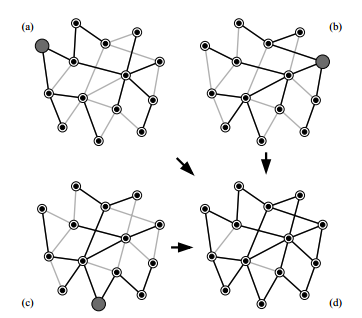
\includegraphics[width=0.5\textwidth]{res/h22.png}
\caption{Tái thiết lập cấu trúc Internet từ kết quả theo dõi: Trong các bảng (a), (b) và (c), ta hiển thị in đậm các cạnh trong ba bộ đường theo dõi bắt đầu đỉnh được tô sáng. Trong bảng điều khiển (d) ta tạo thành sự kết hợp của (a) (b) và (c) để tạo thành một bức tranh về cấu trúc liên kết mạng tổng thể. Lưu ý rằng một vài cạnh bị thiếu trong ảnh(các cạnh màu xám còn lại trong bảng (d)) bởi vì tình cờ chúng không xuất hiện trong bất kỳ ba bộ dữ liệu theo dõi (a) (b) (c).}
\label{fig:h22}
\end{figure}

\section{Cấu trúc Internet}
Khi một người có một tập hợp dữ liệu theo dõi phù hợp, một liên kết đơn giản của tất cả các đường dẫn xuất hiện trong tập dữ liệu sẽ cho chúng ta ảnh chụp nhanh về cấu trúc mạng (Hình \ref{fig:h22} d). Ta đi qua từng đường dẫn và ghi lại đỉnh cho mọi địa chỉ IP xuất hiện trong đường dẫn và cạnh giữa mỗi cặp địa chỉ. Không có khả năng một quy trình như vậy sẽ tìm thấy tất cả các cạnh trong mạng (xem lại hình \ref{fig:h22}d) và đối với các nghiên cứu dựa trên số lượng nguồn nhỏ có thể có sự sai lệch khá nghiêm trọng trong việc lấy mẫu các cạnh . Tuy nhiên, các bộ dữ liệu tốt hơn đang trở nên khả dụng theo thời gian, và người ta tin rằng ta đã đang có một bức tranh hoàn chỉnh hợp lý về hình dạng của Internet.\par
Trên thực tế, hiếm khi có thể thực hiện ghi lại mọi địa chỉ IP trên Internet dưới dạng một đỉnh riêng biệt. Có khoảng 2 tỷ địa chỉ IP được sử dụng trên Internet cùng một lúc, với nhiều địa chỉ xuất hiện và biến mất khi máy tính được bật, tắt hoặc kết nối được hay không được với Internet. Hầu hết các nghiên cứu về Internet đều bỏ qua các máy tính của “người dùng cuối” (End users) và chỉ giới hạn ở các bộ định tuyến, tập trung vào các vùng bên trong và bỏ qua phần ngoài cùng (Hình 2.1). Ở đây ta đề cập đến các Internet như vậy với các đại diện ở cấp độ bộ định tuyến. Các đỉnh trong mạng là các bộ định tuyến và các cạnh giữa chúng là các kết nối mạng.\par
Có vẻ lạ khi bỏ qua các máy tính của người dùng cuối, vì suy cho cùng, họ là toàn bộ lý do cho sự tồn tại của Internet. Tuy nhiên, cấu trúc của mạng ở cấp bộ định tuyến mới chịu trách nhiệm cho hầu hết các khía cạnh về hiệu suất, độ mạnh và hiệu quả của mạng, điều khiển các mô hình lưu lượng trên mạng và tạo thành trọng tâm của hầu hết công việc về cấu trúc và thiết kế Internet, và đó mới là những vấn đề được khoa học quan tâm. Do đó, việc tập trung vào cấu trúc cấp bộ định tuyến là điều hợp lý.\par
\section{Phân nhóm địa chỉ}
Ngay cả sau khi xóa tất cả hoặc hầu hết các máy tính của người dùng cuối khỏi mạng, cấu trúc mạng ở cấp bộ định tuyến vẫn còn quá chi tiết. Thông thường ta muốn một đại diện chi tiết hơn của mạng cung cấp cho ta một bức tranh tổng thể rộng hơn về cấu trúc mạng. Các biểu diễn như vậy được tạo bằng cách nhóm các nhóm địa chỉ IP lại với nhau thành các đỉnh đơn. Ba cách phổ biến để phân nhóm địa chỉ dựa trên ba cách biểu diễn chi tiết khác nhau, ở cấp độ của mạng con, miền và hệ thống tự trị. (subnets, domains, and autonomous systems)\par
Mạng con (subnets) là một nhóm các địa chỉ IP được xác định như sau. Địa chỉ IP bao gồm bốn số, mỗi số trong phạm vi từ 0 đến 255 (8 bit nhị phân) và thường được viết trong một chuỗi, cách nhau bởi dấu chấm. Một khối địa chỉ gồm bốn khối nhỏ dạng “xxx”. Khối cuối là mạng con lớp C, tiếp theo là lớp B và lớp A.\par
Cấp độ cao hơn mạng con là cấp độ miền (domains). Miền là một nhóm máy tính và bộ định tuyến, thông thường kiểm soát bởi một tổ chức và được xác định bởi một tên miền duy nhất, thường là hai hoặc ba phần cuối của địa chỉ máy tính khi được viết dưới dạng văn bản con người có thể đọc. Ví dụ .hust.edu.vn là tên miền của trường Đại họa Bách Khoa Hà Nội. Tên miền của máy tính được xác định một cách đơn giản từ địa chỉ IP của máy tính bằng cách tra cứu DNS, một dịch vụ mạng được thiết lập để cung cấp loại thông tin này. Do đó, với cấu trúc liên kết mạng cấp bộ định tuyến, việc xác định miền mà mỗi bộ định tuyến thuộc và các đỉnh trong mạng theo tên miền là một nhiệm vụ đơn giản.\par
Cấp độ thứ ba là hệ thống tự trị (autonomous systems). Một hệ thống tự trị tương tự như một miền: đó là một nhóm các máy tính, thường nằm dưới sự quản trị đơn lẻ, thường trùng với một miền. Cấp hệ thống tự trị thường không được sử dụng với dữ liệu được lấy theo mẫu traceroute mà với dữ liệu được lấy bằng phương pháp dựa trên các bảng định tuyến BGP, tạo thành đơn vị biểu diễn tự nhiên nhất.\par


\chapter{Cấu trúc Internet sử dụng bảng định tuyến}
Các bộ định tuyến Internet duy trì các bảng định tuyến, cho phép chúng quyết định các gói sẽ được gửi đến đích một cách tốt nhất. Các bảng định tuyến được xây dựng từ thông tin được chia sẻ giữa các bộ định tuyến sử dụng Border Gateway Protocol (BGP). Chúng bao gồm danh sách các đường dẫn hoàn chỉnh từ bộ định tuyến được đề cập đến các điểm đến trên Internet. Khi một gói đến bộ định tuyến, bộ định tuyến sẽ kiểm tra để xác định đích đến của gói và tìm kiếm đích trong bảng định tuyến. Bước đầu tiên của đường dẫn trong bảng nhập thích hợp sẽ cho bộ định tuyến biết gói tin sẽ được gửi đi như thế nào. Trong lý thuyết, bộ định tuyến chỉ cần lưu trữ bước đầu tiên trên mỗi đường dẫn để định tuyến các gói chính xác. Tuy nhiên, để tính toán hiệu quả các tuyến đường sử dụng BGP, ta muốn các bộ định tuyến nhận thức được toàn bộ đường dẫn đến từng điểm đến. Từ ngày đầu cảu Internet, tất cả các bộ định tuyến đã hoạt động bằng cách này. Chúng ta có thể sử dụng việc này để đo cấu trúc của Internet.\par
Các bảng định tuyến trong các bộ định tuyến được thể hiện ở cấp độ của các hệ thống tự trị (autonomous systems -ASes). Khi một gói dữ liệu đến một bộ định tuyến trong một hệ thống tự trị, gói dành cho một máy tính cụ thể trong cùng hệ thống tự trị đó, thì hệ thống tự trị có trách nhiệm đưa gói tin đến đích cuối cùng. Tuy nhiên, dữ liệu truyền giữa các hệ thống tự trị được xử lý bởi cơ chế BGP trên Internet. Do đó, cần để BGP biết về việc định tuyến chỉ xuống mức hệ thống tự trị và các bảng BGP được trình bày thuận tiện nhất theo thuật ngữ hệ thống tự trị. Trong thực tế, các hệ thống tự trị thường trùng với các tên miền, hoặc gần như vậy.\par
Hệ thống tự trị được gán số nhận dạng duy nhất. Đường dẫn định tuyến bao gồm một chuỗi các số AS này bao gồm các đường dẫn đến một số lượng lớn đích, chúng ta có thể tạo một hình ảnh của Internet ở cấp hệ thống tự trị bằng cách kiểm tra chúng. Quá trình này rất giống với quy trình được sử dụng cho phương pháp theo dõi được mô tả trong phần trước, được mô tả trong hình \ref{fig:h22}. Đầu tiên chúng ta có được một số bảng định tuyến. Mỗi bảng định tuyến chứa một số lượng lớn các đường dẫn bắt đầu từ một nguồn duy nhất (bộ định tuyến) và sự kết hợp của các đường dẫn này tạo ra một ảnh chụp mạng tốt nhưng không hoàn chỉnh, trong đó các đỉnh là các hệ thống tự trị và các cạnh là các kết nối giữa các hệ thống tự trị. Như với traceroute, điều quan trọng là các bộ định tuyến được sử dụng phải phân tán tốt trên mạng để tránh trùng lặp quá nhiều kết quả, số lượng bộ định tuyến được sử dụng phải càng lớn càng tốt để lấy mẫu các cạnh mạng càng đầy đủ.\par
\begin{figure}[ht]
\centering
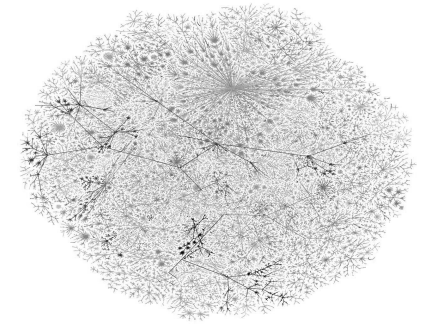
\includegraphics[width=0.5\textwidth]{res/h23.png}
\caption{Cấu trúc của Internet ở cấp độ các hệ thống tự trị. Các đỉnh trong biểu diễn mạng này của Internet là các hệ thống tự trị và các cạnh hiển thị các tuyến đường được lấy bởi dữ liệu truyền đi giữa chúng.}
\label{fig:h23}
\end{figure}


\chapter{Một số hệ thống mạng}
\section{Mạng điện thoại}
Mạng điện thoại, là mạng cố định liên kết không dây, truyền các cuộc gọi điện thoại, là một trong những mạng truyền thông lâu đời nhất vẫn được sử dụng (mặc dù mạng bưu chính chắc cũ hơn), chủ yếu được nghiên cứu bởi các nhà nghiên cứu mạng lý thuyết, vì thường thiếu dữ liệu tốt về cấu trúc của nó. Cấu trúc của mạng điện thoại đã được biết, nhưng dữ liệu phần lớn được các công ty điện thoại sở hữu, chúng không được chia sẻ công khai với cộng đồng nghiên cứu theo cách giống như dữ liệu Internet. Chúng tôi hy vọng rằng tình trạng này sẽ thay đổi, mặc dù vấn đề có thể trở nên khó khăn trong tương lai không xa, vì các công ty điện thoại đang gửi một lượng lưu lượng thoại ngày càng tăng qua Internet thay vì qua các đường dây điện thoại chuyên dụng, và có thể không lâu nữa hai mạng hợp nhất thành một.\par
Một số nguyên tắc hoạt động chung của mạng điện thoại khá là rõ ràng. Ngược lại với Internet, mạng điện thoại truyền thống không phải là chuyển mạch gói. Tín hiệu được gửi qua mạng điện thoại không được phân tách và gửi dưới dạng các gói riêng biệt. Thay vào đó, mạng điện thoại được chuyển mạch kênh, nghĩa là công ty điện thoại có sẵn đường dây hoặc mạch để thực hiện các cuộc gọi điện thoại giữa các điểm khác nhau. Trong những ngày đầu tiên của các hệ thống điện thoại ở Hoa Kỳ và Châu Âu, các đường dây thực sự riêng lẻ, mỗi đường dây là một cuộc gọi, tăng khả năng của mạng, gọi nhiều cuộc gọi hơn là đặt nhiều dây hơn. Tuy nhiên, từ đầu thế kỷ XX, các công ty điện thoại đã sử dụng các kỹ thuật để ghép tín hiệu điện thoại, tức là nhiều cuộc gọi cùng một dây. Cáp điện thoại trong một nhà thường chỉ thực hiện một cuộc gọi mỗi lần, mặc dù điều đó đã thay đổi trong những năm gần đây vì công nghệ mới đã giúp các hộ gia đình có thể có nhiều hơn một số điện thoại và thực hiện nhiều cuộc gọi cùng một lúc.\par
\begin{figure}[ht]
\centering
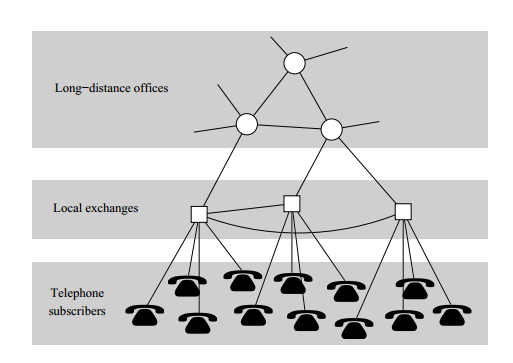
\includegraphics[width=0.5\textwidth]{res/h24.png}
\caption{Sơ đồ cấu trúc ba tầng của mạng điện thoại truyền thống}
\label{fig:h24}
\end{figure}\par
Các hình thức cơ bản của mạng điện thoại là tương đối đơn giản. Hầu hết các quốc gia có mạng điện thoại cố định sử dụng thiết kế ba tầng. Các thuê bao điện thoại cá nhân được kết nối qua các đường dây điện thoại với các tổng đài điện thoại địa phương, sau đó được kết nối qua các đường dây chia sẻ với các văn phòng đường dài (Long-distance offices), đôi khi còn được gọi là văn phòng chuyển mạch (toll-switching offices). Các văn phòng đường dài được kết nối với nhau bằng các đường trung kế (Further trunk lines).(Hình \ref{fig:h24}). Cấu trúc này khá giống với cấu trúc của Internet (Hình \ref{fig:h21}), mặc dù các nguyên tắc hoạt động cơ bản của hai mạng khá khác nhau.\par
Cấu trúc liên kết ba cấp của mạng điện thoại được thiết kế để khai thác các cuộc gọi điện thoại ở hầu hết các địa phương, có nghĩa là chúng kết nối các thuê bao trong cùng thị trấn hoặc khu vực. Các cuộc điện thoại giữa các thuê bao được kết nối cùng địa phương có thể được xử lý chỉ bằng trao đổi mà không cần sử dụng bất kỳ đường trung kế nào cả. Các cuộc gọi như vậy thường được gọi là các cuộc gọi nội hạt (local calls) , trong khi các cuộc gọi đi qua các đường trung kế được gọi là các cuộc gọi đường dài. \par
Mạng điện thoại đã có cấu trúc tương tự như vậy trong hàng trăm năm qua và vẫn còn cho đến ngày nay, chỉ là nhiều chi tiết về cách thức hoạt động của mạng đã thay đổi. Đặc biệt, ở cấp trung kế, một số mạng điện thoại không còn được chuyển mạch kênh. Thay vào đó, giờ đây chúng là các mạng chuyển mạch gói kỹ thuật số hoạt động theo cách khác với Internet, với các cuộc gọi thoại được số hóa, chia thành các gói và truyền qua các liên kết cáp quang. Tuy nhiên, về mặt hình học và cấu trúc liên kết, cấu trúc của mạng điện thoại vẫn giống như trước đây, bị chi phối bởi những hạn chế về địa lý và xu hướng mọi người nói chuyện thường xuyên hơn với những người trong vùng lân cận hơn là với những người ở xa.\par

\section{Lưới điện}
Một mạng lưới điện, trong bối cảnh này, là mạng lưới các đường dây điện cao thế cung cấp vận chuyển điện đường dài trong các quốc gia. Đường dây cung cấp điện cục bộ có điện áp thấp thường được loại trừ. Các đỉnh trong lưới điện tương ứng với các trạm phát và trạm chuyển mạch, và các cạnh tương ứng với các đường dây cao thế. Cấu trúc liên kết của lưới điện không khó để xác định. Các mạng được giám sát bởi một cơ quan duy nhất và bản đồ lưới được hoàn chỉnh sẵn. Thật vậy, dữ liệu về lưới điện rất toàn diện (cũng như các mạng liên quan đến năng lượng khác như đường ống dẫn dầu và khí đốt) có sẵn từ các nhà xuất bản chuyên nghiệp, trên giấy hoặc dưới dạng điện tử cho ai sẵn sàng trả tiền cho chúng.\par
Ta học được nhiều điều thú vị bằng cách nhìn vào cấu trúc của lưới điện. Giống như Internet, lưới điện có khía cạnh không gian, mỗi đỉnh riêng lẻ là một vị trí ở đâu đó trên toàn cầu và sự phân bố của chúng trong không gian rất thú vị từ quan điểm địa lý, xã hội và kinh tế. Thống kê cả về địa lý và cấu trúc liên kết có thể cung cấp cái nhìn sâu sắc về các hạn chế chi phối hình dạng và sự tăng trưởng của lưới điện. Các lưới điện cũng hiển thị một số hiện tượng bất thường, chẳng hạn như sự cố xếp tầng, có thể dẫn đến kết quả tìm được luật của quy mô mất điện.\par
Lưới điện là hệ thống rất phức tạp. Dòng điện không chỉ bị chi phối bởi các định luật vật lý đơn giản mà còn bởi sự điều khiển chính xác và chi tiết các pha và điện áp trên các đường truyền, được theo dõi và điều chỉnh theo thời gian nhanh bởi các hệ thống máy tính tinh vi và thời gian chậm hơn bởi con người. Nó chỉ ra rằng sự cố mất điện và các hiện tượng lưới điện khác bị ảnh hưởng tương đối ít bởi cấu trúc liên kết thô của mạng mà phần nhiều là bởi các hoạt động của nhà điều hành và thiết kế phần mềm.\par

\section{Mạng vận tải}
Một lượng công việc đã được thực hiện trên cấu trúc của các mạng lưới giao thông như đường hàng không, đường bộ và đường sắt. Cấu trúc của các mạng này thường không khó xác định, mặc dù việc biên dịch dữ liệu có thể tốn nhiều công sức. Mạng lưới hàng không có thể được xây dựng từ thời gian biểu của hãng hàng không, mạng lưới đường bộ và đường sắt thì từ bản đồ. Phần mềm hệ thống thông tin địa lý (Geographic information systems -GIS) có thể hữu ích để tăng tốc độ tổng hợp dữ liệu, và cũng có nhiều nguồn tài nguyên trực tuyến cung cấp thông tin hữu ích như vĩ độ và kinh độ của các sân bay.\par
Một trong những ví dụ sớm nhất về một nghiên cứu về mạng lưới giao thông là nghiên cứu của Forge về vận tải đường thủy trên các dòng sông của Nga vào thời Trung cổ. Cũng có một phong trào giữa các nhà địa lý trong những năm 1960 và 70 để nghiên cứu mạng lưới đường bộ và đường sắt, đặc biệt tập trung vào sự tương tác giữa kinh tế và cấu trúc vật lý. Cái tên nổi bật nhất trong phong trào này là của Karel Kansky, và cuốn sách về mạng lưới giao thông của ông là tác phẩm tiêu biểu.\par
Gần đây, một số tác giả đã tạo ra các nghiên cứu áp dụng các ý tưởng phân tích mạng mới cho mạng lưới đường bộ, đường sắt và đường hàng không. Trong hầu hết các mạng được nghiên cứu, các đỉnh đại diện cho các vị trí địa lý và các tuyến đường cạnh giữa chúng. Ví dụ, trong các nghiên cứu về mạng lưới đường bộ, các đỉnh thường đại diện cho giao lộ đường và các đường biên. Nghiên cứu của Sen, mạng lưới đường sắt của Ấn Độ cung cấp một điều thú vị, Sen lập luận rằng, trong bối cảnh du lịch đường sắt, điều quan trọng nhất đối với hầu hết mọi người là liệu có một chuyến tàu trực tiếp đến đích của họ hay không, nếu không, họ sẽ phải đi bao nhiêu chuyến tàu để đến đó. Mọi người không quan tâm quá nhiều đến việc có bao nhiêu điểm dừng trên đường đi, miễn là họ không phải đổi tàu. Do đó, Sen lập luận, một đại diện mạng hữu ích trong trường hợp di chuyển bằng đường sắt là hai đỉnh đại diện vị trí, và hai đỉnh đó được nối với nhau bởi một cạnh nếu một đoàn tàu chạy giữa chúng. Số cạnh bạn cần đi qua để đi từ A đến B bằng với số lượng tàu bạn sẽ phải đi.\par

\section{Mạng giao dịch và phân phối}
Ở giữa mạng lưới giao thông và lưới điện là mạng lưới phân phối, nó được viết tương đối ít trong lĩnh vực nghiên cứu mạng. Mạng lưới phân phối bao gồm những thứ như đường ống dẫn dầu, khí đốt, đường nước, hệ thống thoát nước, các tuyến đường được sử dụng bởi bưu điện, các công ty giao hàng và vận chuyển hàng hóa. Hình \ref{fig:h25} cho thấy một ví dụ, mạng lưới phân phối khí châu Âu, được lấy từ một nghiên cứu của Carvalho, người xây dựng con số từ dữ liệu mua từ các nguồn công nghiệp. Trong mạng này, các cạnh là các đường ống dẫn khí và các đỉnh là giao điểm của chúng, bao gồm bơm, chuyển mạch, và các cơ sở lưu trữ và nhà máy lọc dầu.
\begin{figure}[ht]
\centering
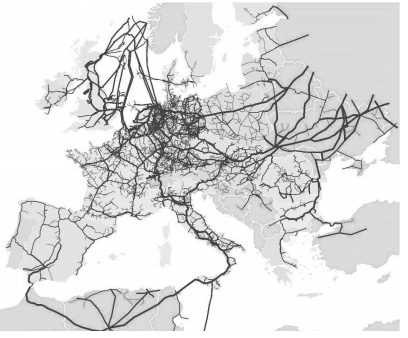
\includegraphics[width=0.5\textwidth]{res/h25.png}
\caption{Mạng lưới đường ống khí đốt ở Châu Âu.}
\label{fig:h25}
\end{figure}\par
Nếu một người muốn giải thích sự phân phối một cách đơn giản, có một loại mạng phân phối đã được nghiên cứu khá tốt là mạng sông (river networks), mặc dù mạng sông chính xác hơn là một mạng thu thập thay vì là mạng phân phối. Trong một mạng sông, các cạnh là sông hoặc suối và giao điểm của chúng là các đỉnh. Giống mạng lưới đường bộ, không có kĩ thuật đặc biệt nào để thu thập dữ liệu về cấu trúc mạng sông. Công việc khảo sát đã được thực hiện bởi khảo sát viên và người vẽ bản đồ, tất cả những gì ta làm chỉ là sao chép kết quả từ bản đồ ra.
\begin{figure}[ht]
\centering
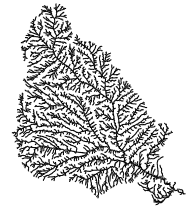
\includegraphics[width=0.5\textwidth]{res/h26.png}
\caption{Lưu vực thoát nước ở Loess Plateau: Mạng lưới sông suối trên Loess Plateau ở Sơn Tây tỉnh của Trung Quốc. Nhìn thấy được trong cấu trúc giống như cây của mạng là không có vòng lặp, vì vậy nước tại bất kỳ điểm nào trong mạng đều có một đường để thoát ra}
\label{fig:h26}
\end{figure}\par


\end{document}

